%\section{Introduction}
%\par The importance of quality calibration for this work is mainly justified by skepticism towards the camera's factory calibration and the quality of the used software. Because the camera's software presents big constraints and brings large sources of mistakes with unknown origins, the best way to process the results is to obtain the RAW data and treat it resorting to a special made Matlab code and a blackbody calibration. \\
\section{Blackbody Calibration Sources}
\par Black Body Calibration sources are recommended by the camera manual to calibrate the camera correctly. They are simply blackbodies with controllable temperature. The temperature controlled blackbody is to be filmed by the IR Camera and the camera's raw data (signal intensity received by the sensors) extracted. With a known temperature and high emissivity it is easy to correlate the signal intensity with the correspondent temperature. Establishing this relation can be done directly in the software but for the aforementioned reasons this was the procedure established and developed in this work.\\

\par The Blackbody Calibration Source is the name given to these devices, that are commercialized to calibrate infrared sensors. Given the high costs of these devices (over 7000 euros) a simple but functional Blackbody Calibration Source was projected and assembled in the present work.\\

\par There are several types of blackbody calibration sources, which are included in these main categories \cite{blackbody}: 
\begin{itemize}
\item Fixed-Point Blackbody Radiators: used at really high temperatures (>1000ºC), these are characterized by having a metal (eg. Au, Ag or Cu) at freezing point and a graphite made cavity (high emissivity). The quality of the measure is defined by the quality of the graphite, metal ingot and shape of the cavity.
\item Heat Pipe Cavities: used for applications with temperatures from -60ºC to 1000ºC, depending on the working fluid, these are characterized by having the best precision and being the most sophisticated devices. The cavity is surrounded by a multistate heated fluid at a controlled pressure. This cavity has special geometric properties to enhance the emissivity of the body. They are usually used in high precision applications for instance in meteorology institutes.
\item Pratical Cavities: used in more pratical applications, they are used for a range of temperatures between -45ºC and 450ºC. Unlike the Heat Pipe, the working fluid rarely changes its physical state (eg. one could only go up until 100ºC with water). Pratical cavities are easy to build and are often used for tests by radiation thermometers manufacturers. Similarly to the Heat Pipe Cavities also rely on specific geometric conditions to enhance the cavity's emissivity.
\item Flat Plate: these devices are used as an alternative to the pratical cavities because they do not require small cavities. As counterpart of in these devices, the heated plate must have a high emissivity, usually obtained using a high emissivity paint, so they may lead o large uncertainties. This method is usually used for large applications which do not require very accurate measurements.
\item Others: Cryogenic/Vaccum Blackbodies are used for extreme values of temperature such as negative temperatures ( as low as -100ºC) and Furnaces used in this case as a Flat plate for temperatures above 1000ºC.
\end{itemize}

\par For this work, the Pratical Cavity Radiator is the best choice, not only because it's often used for similar applications, within the same temperature range, but also because it is the simplest solution to build. The final design of the chamber was based on the scheme presented in Hartmann's work \cite{blackbody}, and it's illustrated in Figure \ref{fig:bbs}. The cavity shape is based on the design proposed in Figure \ref{fig:blkbody}. Since the camera had to be calibrated to work between 0 and 130ºC, the working fluid selected here was oil, with high saturation temperatures (300ºC at atmospheric temperature). \\

\begin{figure}
\centering
\includegraphics[width=0.6\linewidth]{Figures/4.Chapter/praticalcavity.png}
\caption{Pratical Cavity Blackbody Source scheme}
\source{Chapter 3.2 from \cite{blackbody}}
\label{fig:bbs}
\end{figure}


\par The effect of the cavity shape show in Figure \ref{fig:blkbody} is used in many cavity based Blackbody Radiator Devices and is used to enhance the emissivity, by trapping the light, thus reducing the light reflected from the outside. This effect is enhanced by an angle of 30º as referenced in the literature \cite{blackbody}. A working scheme of the final design of the created device, with a mixture of these 2 concepts is presented in Figure \ref{fig:box}. \\

\begin{figure}[h]
\centering
\includegraphics[width=0.6\linewidth]{Figures/4.Chapter/blackbody3.jpg}
\caption{Cavity and light trapping effect scheme}
\source{NASA}
\label{fig:blkbody}
\end{figure}

\begin{figure}[h]
\centering
\includegraphics[width=0.6\linewidth]{Figures/4.Chapter/caixa.png}
\caption{Final design scheme for the Blackbody Calibration Source}
\label{fig:box}
\end{figure}

\subsection{Design details}
\par The final design render, made in SolidWorks, is depicted in Figure \ref{fig:render}. One may notice, both from the render and the scheme, that the box is too long compared to the blackbody. The reason for this is that the whole device had to be made to fit the thermal resistances which were commercially available. This resistance is presented in Figure \ref{fig:res}. The working fluid must have good conductive properties, so the type of oil used was car oil, which is stable under heating conditions. \\

\begin{figure}[h]
\centering
\includegraphics[width=0.8\linewidth]{Figures/4.Chapter/caixa_render.PNG}
\caption{SolidWorks render of a cut device view}
\label{fig:render}
\end{figure}

\par In both the scheme and render, the sensors, peripherals of the device and its insulation are omitted. Five type K thermocouples were used: 2 submerse thermocouples by each side of the blackbody to check if there were high temperature variations in different regions of the device; 3 surface thermocouples to monitor when the temperature stabilizes in the face of the device that is recorded by the IR camera (for the calibration procedure), and to provide enough temperature measurements from which one could take a good average of the real cavity temperature. The positioning of the thermocouples is schematically depicted in Figure \ref{fig:tpar}. \\

\begin{figure}[h]
\centering
\includegraphics[width=0.9\linewidth]{Figures/4.Chapter/resistencia.png}
\caption{Thermal Resistance used}
\label{fig:res}
\end{figure}

\begin{figure}[h]
\centering
\includegraphics[width=0.9\linewidth]{Figures/4.Chapter/termopares.png}
\caption{Thermocouple placement scheme}
\label{fig:tpar}
\end{figure}

\par A KS 20-1 PID controller, that controls the resistance based on the temperature monitored by the middle surface thermocouple and a DT9828 Data Acquisition Board from Data Translation to connect the thermocouples to the computer were the data is processed.\\

\par Finally, the insulation consists of a 5mm PENA30FR adhesive, that is composed by sponge with aluminum coating. This material can be seen in Figure \ref{fig:isola}. The insulation is used all around the device and the only hole in it is the opening for the blackbody. \\

\begin{figure}[h]
\centering
\includegraphics[width=0.5\linewidth]{Figures/4.Chapter/insulation.jpg}
\caption{PENA30FR Adhesive Insulation}
\label{fig:isola}
\end{figure}

\subsection{Building Process}

\par The building process of this device can be divided in 4 parts:

\begin{itemize}
\item The box: made in stainless steel, this box had to be ordered from a company specialized in metal work. The size of this box is 200x200x320 mm, with 2mm thickness. It already has 2 orifices to assemble the resistance and the blackbody. Thermal insulation was made to fit the box measures. The box is insulated only when both the blackbody and resistance are already installed.
\item The resistance: bought from Mecafil, has a power of 1500W and was attached to the box with the help of a nut (glued to the back with cold weld). The hole used to accommodate the electrical resistance is also used to fill in and drain the device with the oil. The junction between the nut and the bolt was also reinforced with high temperature silicone, and the screw of the resistance was covered with a Teflon tape to avoid leakages.
\item The blackbody: is made by laser cut from a 1mm stainless steel plate, painted with a black matte paint, then bent and finally welded. After the weld, the blackbody had to be re-painted and its insulation reinforced with high temperature silicone. Finally it had to be screwed to its support plate so it could be placed in the box. The end result can be seen in Figure \ref{fig:blkbdy}. This piece was made removable so that new shapes could be made, giving room to the future improvements of the device. When placed on the device it is important to put some high temperature silicon to fully prevent any leakages.
\item The peripherals: starting with the sensors, holes were made on the top of the box so that every sensor could pass through it. The scheme for the holes and the sensors display was already shown in Figure \ref{fig:tpar}. The Data Acquisition Board and the PID controller need to be placed near the box because of the sensor wire length restraint, so a support was made to accommodate everything.
\end{itemize}

\begin{figure}[h]
\centering
\includegraphics[width=0.7\linewidth]{Figures/4.Chapter/blackbody.png}
\caption{Completed Blackbody}
\label{fig:blkbdy}
\end{figure}

\par The final setup, after all parts were mounted can be seen in Figure \ref{fig:bbcs}. With this setup, it is possible to collect and control temperature values, and correlate them with the camera data. This device was used to perform 2 different calibrations, that will be explained further ahead in this chapter. \\

\begin{figure}[h]
\centering
\includegraphics[width=0.7\linewidth]{Figures/4.Chapter/complete.png}
\caption{Completed Blackbody Calibration Source: (1) Blackbody cavity; (2) Data Aquisition Board; (3) PID controller; (4) IR Camera; (5) Thermocouples (one connected to the PID, the others to the Data Aquisition Board)}
\label{fig:bbcs}
\end{figure}

\section{Calibration process}

\par A number of steps must be followed before starting the actual calibration process:
\begin{itemize}
\item Fill the device with oil.
\item Connect the thermocouples to the Data Aquisition Board and to the PID Controller.
\item Turn on the IR Camera and start both its software (Xeneth) and the board software (QuickDAQ).
\item Define an adequate integration time to the desired temperature interval.
\item Perform an offset calibration with the camera software.
\end{itemize}

\par Now the camera can be calibrated using the software’s calibration feature or the custom made process proposed here. While in the software calibration is automatic, in the custom made calibration the average ADU of the selected region needs to be registered along with the average temperature read by the sensors on an Excel sheet. \\

\begin{figure}[h]
\centering
\includegraphics[width=0.55\linewidth]{Figures/4.Chapter/calibinprog.jpg}
\caption{Calibration Instalation in Function}
\label{fig:calibinprog}
\end{figure}

\begin{figure}[h]
\centering
\includegraphics[width=1\linewidth]{Figures/4.Chapter/ex11.png}
\caption{Blackbody thermal image and its respective histogram}
\label{fig:ex1}
\end{figure}

\par The overall setup for the custom made calibration is assembled in Figure \ref{fig:calibinprog}. The desired temperature is set and is gradually increased in 10ºC/20ºC increments to have a wide range of temperatures (up to 130ºC).Each set temperature must stabilize until the image of the cavity shows a uniform temperature within the entire selected area. For instance, Fig. 4.11 shows that the edges of the cavity are hotter than the remaining cavity region. This is due to different thermal properties of the materials used to assemble the cavity blackbody.\\

\par This problem is solved by the PID controller. To understand this, one can summarize the way the PID is working to control the temperature as follows: the input target temperature of the PID is compared with that read by the thermocouple connected to the controller, and it turns on and off the resistance to keep the temperature constant within a desired range (+/-1ºC). The resistance is turned of just before the oil is at the desired temperature in order to account for thermal inertia of the device and for the delays in the controller.\\

\begin{figure}[h]
\centering
\includegraphics[width=0.9\linewidth]{Figures/4.Chapter/ex2.png}
\caption{Calibration example: initial temperature field, and uniform temperature field (after $\approx$5 min)}
\label{fig:ex2}
\end{figure}

\par So, when the electrical resistance is off, the thermal inertia of the oil and the good insulation of the Blackbody device allow reaching a uniform temperature in the cavity, as the device cools down. This can be clearly seen in Fig. 4.12.
The histograms show perfectly the desired conditions (the peak on the right histogram contrasting with the wider dispersion of values in the left histogram in Figure \ref{fig:ex2}). \\

\par To see what temperature corresponds to the averaged ADU value, an average of the surface thermocouple read temperatures in time was taken, with the help of the software QuickDAQ, which allows to take a data sample for a fixed amount of time. This is used to make the average between all the surface thermocouples connected to the board and the value shown in the PID. This final average is then the input for the software calibration or saved with the ADU in an excel for the second method. \\

\subsection{Software Calibration}

\par The Xenics' software has a camera calibration wizard (in which the offset calibration feature is included) that automatically correlates the ADU's with the temperature measured. The feature described is called "Temperature Calibration (Plank)" and can be seen in Figure \ref{fig:plankcalib}. In the shown interface, the user can input the temperature measured by the thermocouples in the field (a), and then add the read value with button (b). It will then add a point, to the table at the left and draw in on a graph bellow. This point has the given temperature, and the ADU measured with a spatial average of a small rectangular area in the center of the image. \\

\begin{figure}[h]
\centering
\includegraphics[width=0.7\linewidth]{Figures/4.Chapter/plankcalib.png}
\caption{Xeneth's software - Temperature Calibration (Plank)}
\label{fig:plankcalib}
\end{figure}

\par In the first calibration, this method was tried but because the temperature and respective measured ADU are shown it didn't invalidate the possibility to use them in the second method, our custom made calibration. In this attempt an integration time of 450 was used. The final table and graphic can be seen in Figure \ref{fig:calib}. On the table labeled as (a) one can see 5 columns. The first and last columns depict the read values of temperature and ADU, respectively. The second and third columns show the ambient temperature and emissivity which are actually irrelevant for the present calibration as one assumes the cavity to be a perfect blackbody, so the ambient temperature won't be used in this calibration. The fourth column is a variable, which depends on the input temperature, that the software uses to convert, together with the other inputs, the temperature, in a quantity called "Soaled Radiance", represented in the x axys of graph (b) in Figure \ref{fig:calib}. This variable is not explained in the manual, nor its relation with the temperature. This was one of the disadvantages of this method mainly because the software creates the "Soaled Radiance" value out of it, and it is supposed to maintain a proportional relation with the ADU's so the calibration correlation is linear. But as it is noticeable in the graph, the values do not follow the line that closely, which caused a significant deviation. \\

\par Having this variable and the "Soaled Radiance" unexplained, the only option was to take these values and use them in the other method. Another reason is that this method does a linear correlation. This may only be a vague assumption or a rough approximation, and because even if the origin of these variables was known, there would be no way to validate that linear relation. \\

\par In the end, the software creates a calibration conversion that can be selected when it is opened and used to take the data directly in Celsius. This calibration file can only be used for the specified integration time. In Figure \ref{fig:calib} it's possible to see how the software approximates linearly (green line) the measured points (red line). Because this calibration didn't match the experimental values as close as desired, when the newly created calibration pack was tested it didn't work properly, so the second type of calibration was made.\\

\begin{figure}[h]
\centering
\includegraphics[width=0.7\linewidth]{Figures/4.Chapter/calibracao.png}
\caption{Complete Temperature Calibration (Plank)}
\label{fig:calib}
\end{figure}

\subsection{Proposed Calibration}
\par Being unable to trust the calibration method provided by the camera software, a custom made method was developed. In this method the calibration results (average ADU in a selected region) are taken directly from the software, without using the software's Calibration Wizard. They're saved in an Microsoft Excel sheet together with the average temperature read by the thermocouples. With this method the results have to be taken raw from the software and then process them with the MATLAB code that was made just for this purpose. A whole explanation of the process will be given in the next section, leaving in this section a general outline of the proposed method.\\

\par The process of data aquisition for the calibration is similar to the previous calibration. The main difference in this method is the absence of the Calibration Wizard. Instead, the Selection Panel (described in \ref{software}) is used to gather the average measured ADU of a circular area, similar to what can be seen in Figure \ref{fig:ex2}. There are several advantages in this method, one being that it was now possible to adjust the temperature range (the Calibration Wizard didn't allow it), and better understand when the image saturates. Another advantage is the fact that it is possible to change integration time. \\

\par In Microsoft Excel, the measured temperatures are converted into the radiated energy using equation \ref{eq:6} (and considering the object perfectly black) and plotted against the ADU. Then Microsoft Excel's trending line function is used to extract a polynomial curve that will best approximate the data gathered in the experiments. The second and third degree polynomial approximations were compared, but in the end the third degree polynomial. This option took longer to process but the end result was significantly closer to the experimental results. \\

\par With the extracted curve a MATLAB code was made to calibrate the videos. The raw data video data (in ADU) matrix is the input of this function. This matrix has the value for every pixel in every frame, and point by point is solving the following equation:

\begin{equation}
A \times W_{tot}^3 + B \times W_{tot}^2 + C \times W_{tot} + D = ADU_{pixel}
\end{equation}

in which A,B,C and D are the coefficients of the calculated polynomial curve, $ADU_{pixel}$ is the pixel ADU value and $W_{tot}$ is the wanted radiated energy. Using this radiated energy value, the pixel temperature is calculated using equation \ref{eq:7}. The end result is a matrix with all the temperatures.

\subsection{Calibration Process Details}

\par One important fact about the designed calibration procedure is that it took a whole day to complete. This is due to the fact that there was no refrigeration system and the liquid had to cool at room temperature. Also the overheating of the device often leads to leakages due to material expansion and break down. This problem, which often would not allow to repeat the calibration process in a regular way, took some time to address.\\

\par Two calibrations were made during this work. The first was made using the software at the fixed integration time of it=450us. The second was made using the proposed method for the integration times of it=450us and it=200us. With the integration time of it=450us the image would saturate at around 108ºC, so the correspondent results weren't suited for the experiments represented here which would reach higher temperatures. \\

\par The results of the calibrations is shown in Table \ref{tab:calibration}. Since the results were taken for both calibrations at $it=450us$ we can use them to prove the method's consistency. The comparison is presented Figure \ref{fig:calibplot}.  \\

\begin{table}[h]
\centering
\caption{Calibration Results}
\label{tab:calibration}
\begin{tabular}{ccccccccc}
\toprule
\multicolumn{3}{c}{Calibration 1}       &  & \multicolumn{5}{c}{Calibration 2}                                    \\ 
\cmidrule[0.4pt](r{0.125em}){1-3}%
\cmidrule[0.4pt](r{0.125em}){5-9}%
         & \multicolumn{2}{c}{it=450us} &  &        & \multicolumn{2}{c}{it=450us} & \multicolumn{2}{c}{it=200us} \\
\cmidrule[0.4pt](r{0.125em}){2-3}%
\cmidrule[0.4pt](r{0.125em}){6-7}%
\cmidrule[0.4pt](r{0.125em}){8-9}%
T(ºC)  & ADU         & $W_{tot}(W/m^2)$      &  & T(ºC)& ADU         & $W_{tot}(W/m^2)$      & ADU         & $W_{tot}(W/m^2)$      \\
\cmidrule[0.4pt](r{0.125em}){1-3}%
\cmidrule[0.4pt](r{0.125em}){5-9}%
25.5     & 3141        & 450.1533       &  & 25.46  & 3200        & 449.912        & 1645        & 449.912        \\
41       & 4246        & 551.1904       &  & 34.5   & 3794        & 506.9481       & 1900        & 506.9481       \\
49       & 4879        & 609.5461       &  & 44.28  & 4666        & 574.5844       & 2285        & 574.5844       \\
68.5     & 7142        & 771.1625       &  & 62.27  & 6287        & 716.4103       & 3021        & 716.4103       \\
86.6     & 9928        & 948.1167       &  & 75.76  & 8270        & 838.8605       & 3890        & 838.8605       \\
108      & SAT         & SAT            &  & 84.33  & 9827        & 924.4022       & 4596        & 924.4022       \\
         &             &                &  & 94.54  & 12094       & 1034.669       & 5586        & 1034.669       \\
         &             &                &  & 103.67 & 14078       & 1141.372       & 6690        & 1141.372       \\
         &             &                &  & 114.39 & SAT         & SAT            & 8139        & 1276.958       \\
         &             &                &  & 125.74 & SAT         & SAT            & 9885        & 1433.317     \\ \bottomrule
\end{tabular}
\end{table}

\begin{figure}[h]
\centering
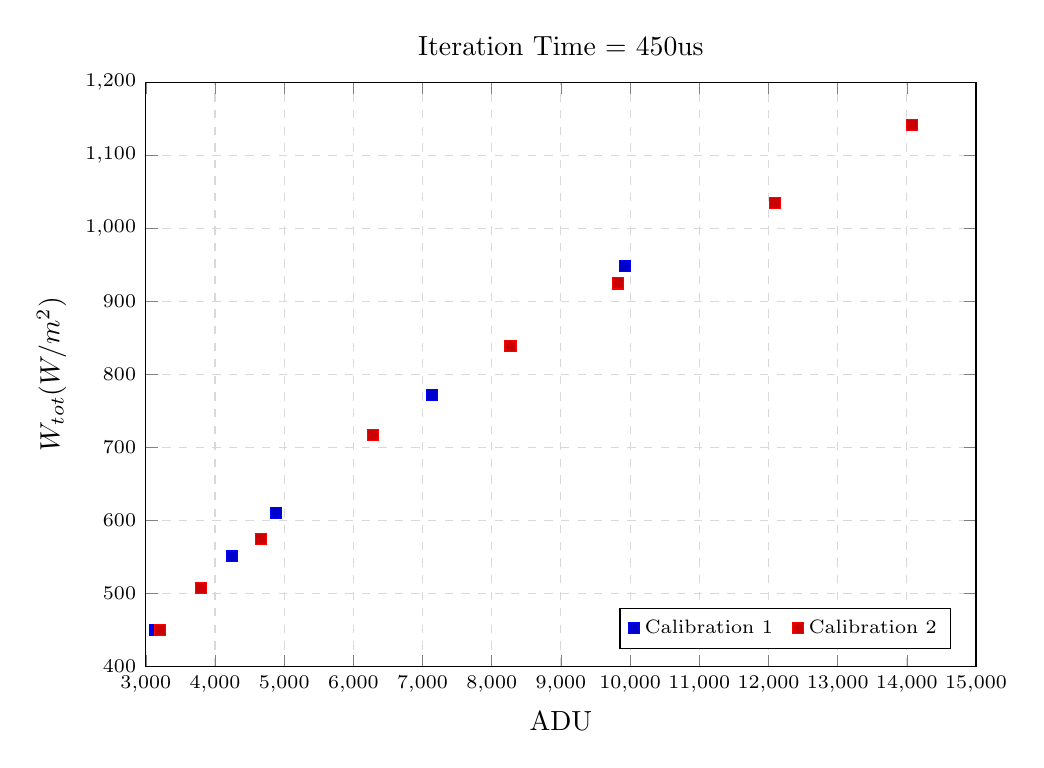
\begin{tikzpicture}
\begin{axis}[
	title = {Iteration Time = 450us},
    tick label style={font=\scriptsize},
    legend style={font=\scriptsize,/tikz/column 2/.style={column sep=5pt},},
    legend columns=2,
    legend cell align=left,
	legend pos =south east,
    grid=major, % Display a grid
    grid style={dashed,gray!30}, % Set the style
    xlabel={ADU},
    ylabel={$W_{tot} (W/m^2)$}, 
    ymin = 400, ymax = 1200,
    %ytick={300,325,350,375,400,425,450,475,500,525},
    %yticklabels={300,325,350,375,400,425,450,475,500,525},
    xmin = 3000, xmax = 15000,
    xtick={0,1000,...,15000},
    xticklabel style={
        /pgf/number format/fixed,
        /pgf/number format/precision=5},
	scaled x ticks=false,
    width=\textwidth, height=9cm,
    %legend entries={Experimental,Computational, $264 W/m^{2}$,$807 W/m^{2}$,$2031 W/m^{2}$,$3636 W/m^{2}$}
    ]

% \addlegendimage{only marks, mark=square*,black}
% \addlegendimage{only marks, mark=x      ,black}
% \addlegendimage{only marks, mark=*      ,blue}
% \addlegendimage{only marks, mark=*      ,red}
% \addlegendimage{only marks, mark=*      ,brown}
% \addlegendimage{only marks, mark=*      ,black}


%-------------------------------------------------------------
%Experimental ------------------------------------------------
%-------------------------------------------------------------

\addplot+[only marks,mark=square*,blue] % 264 experimental
coordinates {(	3141	,	450.1532612	)
(	4246	,	551.1904079	)
(	4879	,	609.5460842	)
(	7142	,	771.1624794	)
(	9928	,	948.1166888	)
};
\addplot+[only marks,mark=square*,red]
coordinates{(	3200	,	449.9120215	)
(	3794	,	506.9481463	)
(	4666	,	574.5844207	)
(	6287	,	716.4103256	)
(	8270	,	838.8604805	)
(	9827	,	924.4022127	)
(	12094	,	1034.669156	)
(	14078	,	1141.371929	)};
\legend{Calibration 1, Calibration 2}

\end{axis}
\end{tikzpicture}
\caption{Comparison of the two calibrations at it=450us}
\label{fig:calibplot}
\end{figure}

\par Next, the $it=200us$ data has to be plotted, and a trending line calculated. The data with the correspondent trending line can be seen in Figure \ref{fig:calibcurve}. The equation that is represented in the plot is the one used in the calibration code. \\

\begin{figure}[h]
\centering
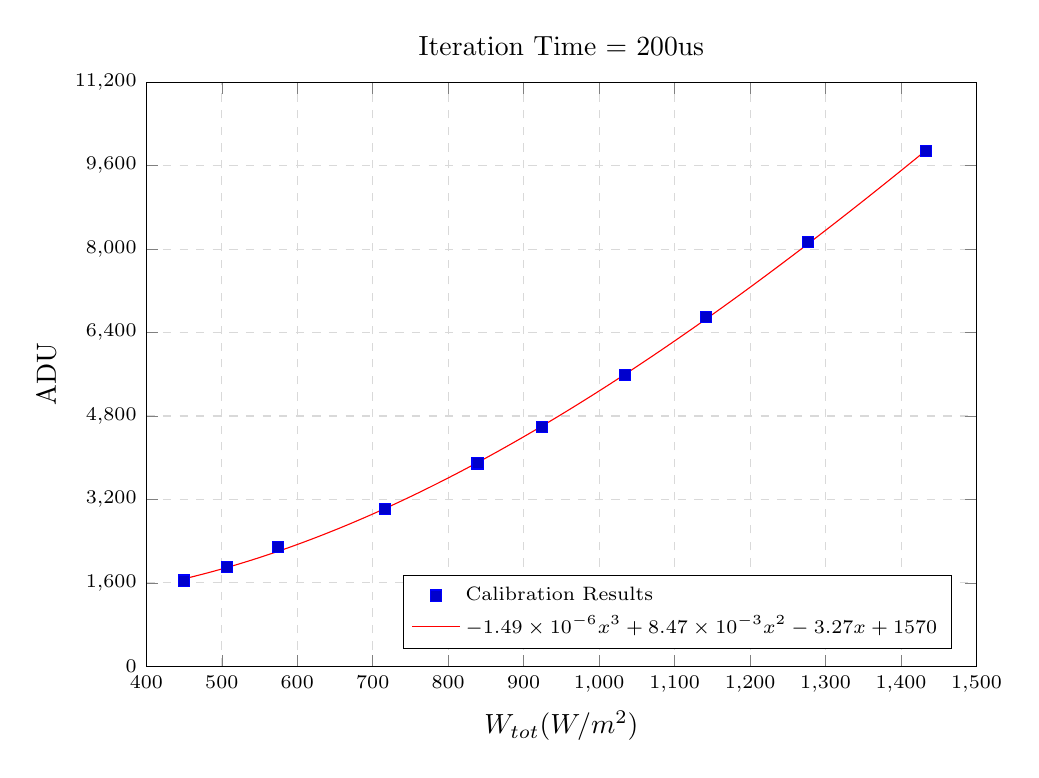
\begin{tikzpicture}
\begin{axis}[
	title = {Iteration Time = 200us},
    tick label style={font=\scriptsize},
    legend style={font=\scriptsize,/tikz/column 2/.style={column sep=5pt},},
    %legend columns=2,
    legend cell align=left,
	legend pos =south east,
    grid=major, % Display a grid
    grid style={dashed,gray!30}, % Set the style
    xlabel={$W_{tot} (W/m^2)$},
    ylabel={ADU}, 
    ymin = 0, ymax = 11200,
    %ytick={300,325,350,375,400,425,450,475,500,525},
    %yticklabels={300,325,350,375,400,425,450,475,500,525},
    xmin = 400, xmax = 1500,
    ytick={0,1600,...,11200},
    yticklabel style={
        /pgf/number format/fixed,
        /pgf/number format/precision=5},
	scaled y ticks=false,
    width=\textwidth, height=9cm,
    ]
\addplot+[only marks,mark=square*,blue]
coordinates {(	449.9120215	,	1645	)
(	506.9481463	,	1900	)
(	574.5844207	,	2285	)
(	716.4103256	,	3021	)
(	838.8604805	,	3890	)
(	924.4022127	,	4596	)
(	1034.669156	,	5586	)
(	1141.371929	,	6690	)
(	1276.958202	,	8139	)
(	1433.317083	,	9885	)
};
\addlegendentry{Calibration Results}
\addplot[
    domain=450:1430, 
    samples=100, 
    color=red,
]{0.00847*x^2 - 0.00000149*x^3 - 3.27*x + 1570};
\addlegendentry{$-1.49\times 10^{-6}x^3 + 8.47\times 10^{-3}x^2 - 3.27x + 1570$}
\end{axis}
\end{tikzpicture}
\caption{Comparison of the two calibrations at it=450us}
\label{fig:calibcurve}
\end{figure}

\par The generated code is used to transform every video from ADU values to Celsius, and works only for the selected integration time. The code can also be easily adapted to the integration time of 450us. This code can be seen in Appendix \ref{ap:a}. \\

\clearpage

\section{Data Processing Methods}
\par The collected images, without any sort of treatment, have some random noise and unwanted patterns of noise. While the noise source is usually small differences in sensitivity or calibration of the sensors, the patterned noise has it's origin mainly on the software processing. A temperature difference is always noticeable inside the region of interest. This cannot be solved so, to accurately evaluate the results, a background remove has to be performed. This also helps removing some background noise. \\

\par To be treated, the video needs to be imported to avi format, in an 8 bit, grey scale format. In MATLAB, the video is divided into frames and the grey scale value transformed to temperature, considering the temperature or ADU scale it was imported with. After this, the calibration is applied and finally the filters. In the end, the results are extracted as a MATLAB file with all values and a txt with the results from the center to the radius of the droplet with a plot option.

\subsection{Patterned Noise}

\par The origin of this type of noise was detected in the software's zoom function. It can result in significant errors. At constant temperature the results showed that the  difference between pixels side by side was 1ºC. To remove this, a filter was made that would add and subtract 0.5ºC alternately. The generated pattern and the effect of the filter can be seen in Figure \ref{fig:chess}.

\begin{figure}[h]
\centering
\includegraphics[width=0.5\linewidth]{Figures/4.Chapter/chess2.png}\\
\subfigure{
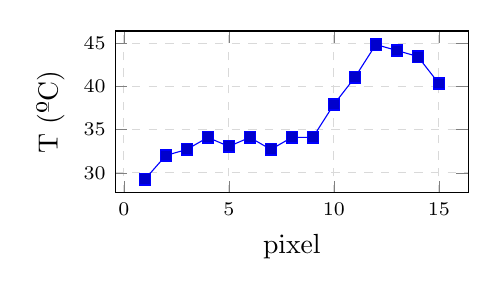
\begin{tikzpicture}
\begin{axis}[
	width=0.5\linewidth,
    height=0.3\linewidth,
	%title = {Unprocessed Results},
    tick label style={font=\scriptsize},
    legend style={font=\scriptsize,/tikz/column 2/.style={column sep=5pt},},
    %legend columns=2,
    legend cell align=left,
	legend pos =south east,
    grid=major, % Display a grid
    grid style={dashed,gray!30}, % Set the style
    xlabel={pixel},
    ylabel={T (ºC)}, 
    %ymin = 0, ymax = 11200,
    %ytick={300,325,350,375,400,425,450,475,500,525},
    %yticklabels={300,325,350,375,400,425,450,475,500,525},
    %xmin = 400, xmax = 1500,
    %ytick={0,1600,...,11200},
    %yticklabel style={
    %    /pgf/number format/fixed,
    %    /pgf/number format/precision=5},
	%scaled y ticks=false,
    ]
\addplot+[mark=square*,blue]
coordinates {(	1	,	29.23	)
(	2	,	32	)
(	3	,	32.7	)
(	4	,	34.09	)
(	5	,	33.05	)
(	6	,	34.09	)
(	7	,	32.7	)
(	8	,	34.09	)
(	9	,	34.09	)
(	10	,	37.9	)
(	11	,	41.03	)
(	12	,	44.84	)
(	13	,	44.15	)
(	14	,	43.45	)
(	15	,	40.33	)
};
%\addlegendentry{}
\end{axis}
\end{tikzpicture}
}%
\subfigure{
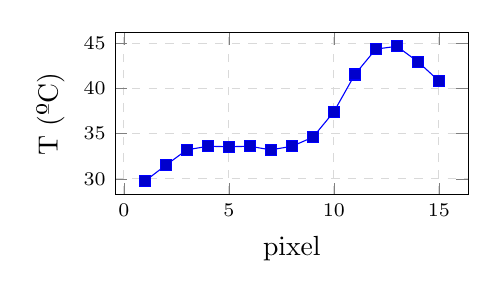
\begin{tikzpicture}
\begin{axis}[
	width=0.5\linewidth,
    height=0.3\linewidth,
	%title = {Processed Results},
    tick label style={font=\scriptsize},
    legend style={font=\scriptsize,/tikz/column 2/.style={column sep=5pt},},
    %legend columns=2,
    legend cell align=left,
	legend pos =south east,
    grid=major, % Display a grid
    grid style={dashed,gray!30}, % Set the style
    xlabel={pixel},
    ylabel={T (ºC)}, 
    %ymin = 0, ymax = 11200,
    %ytick={300,325,350,375,400,425,450,475,500,525},
    %yticklabels={300,325,350,375,400,425,450,475,500,525},
    %xmin = 400, xmax = 1500,
    %ytick={0,1600,...,11200},
    %yticklabel style={
    %    /pgf/number format/fixed,
    %    /pgf/number format/precision=5},
	%scaled y ticks=false,
    ]
\addplot+[mark=square*,blue]
coordinates {(	1	,	29.73	)
(	2	,	31.5	)
(	3	,	33.2	)
(	4	,	33.59	)
(	5	,	33.55	)
(	6	,	33.59	)
(	7	,	33.2	)
(	8	,	33.59	)
(	9	,	34.59	)
(	10	,	37.4	)
(	11	,	41.53	)
(	12	,	44.34	)
(	13	,	44.65	)
(	14	,	42.95	)
(	15	,	40.83	)
};
%\addlegendentry{}
\end{axis}
\end{tikzpicture}
}
\caption{The effect of the filter in both the image and a line of point temperature values}
\label{fig:chess}
\end{figure}


\subsection{Median Filter}

\par This filter has the potential to remove random bad pixels noise from the picture. This filter is a MATLAB function that outputs the median of a 3-by-3 neighborhood of the input pixel. With this simple filter the image can be greatly improved as shown in Figure \ref{fig:median}. On the right there's the image without the filter and on the left the treated image.

\begin{figure}[h]
\centering
\includegraphics[width=0.6\linewidth]{Figures/4.Chapter/median.png}
\caption{Median filter effect}
\label{fig:median}
\end{figure}

\subsection{Background Filter}
\par The background filter serves the function of eliminating any problems related with the optics of the camera and to equalize the temperature field. Two different ways to do it were thought. Two MATLAB codes were made and tested. The first one is the simple way and is shown in Equation \ref{eq:bkg}. The variable $vid$ is the matrix with the temperature value for every pixel in every frame, $avTemp$ is the average temperature in the center of the hole and $t_n$ is the number of the analyzed frame.
\begin{equation}\label{eq:bkg}
vid^{*}(x,y,t_n)=vid(x,y,t_n)-vid(x,y,1)+avTemp
\end{equation}
\par The second one is a weighted background removal and we can see it in Equation \ref{eq:pbkg}. The variables bear the same meaning, but has to be done for each pixel ($x_p,y_p$). Only the code for the latter can be seen in Appendix \ref{ap:b} as the code is similar in both cases. 
\begin{equation}\label{eq:pbkg}
vid^{*}(x_p,y_p,t_n)=\frac{vid(x_p,y_p,t_n)-vid(x_p,y_p,1)}{vid(x_p,y_p,1)}avTemp+avTemp
\end{equation}
\begin{figure}[h]
\centering
\includegraphics[width=0.8\linewidth]{Figures/4.Chapter/bkg.png}
\caption{Background filter effect}
\label{fig:bkg}
\end{figure}

\subsection{Heat Flux computation}

\par To evaluate and compare the heat removal capacity of the system it is very important to compute the heat flux and cooling effectiveness, mentioned in Section \ref{sec:heat}. This was also made with the help of a MATLAB code, that can be seen in Appendix \ref{ap:c} and \ref{ap:d}.\\
\par Starting with the computation of the heat flux the code is a discretization of Equation \ref{eq:heatf}. This equation can be divided in three terms: the provided heat flux, the spacial term and the temporal term. This problem was addressed as being axisymmetric, so the spatial derivative becomes a one-dimensional problem. To address the second order derivative in the spatial term a backward discretization with first order precision was applied:\\
\begin{equation}
\frac{{\partial}^2 T}{\partial r^2} \approx \frac{T_i-2T_{i-1}+T_{i-2}}{\Delta r^2}
\end{equation}

\par The temporal term has a first order derivative, that was addressed the same way and discretized using a first order precision backward method:

\begin{equation}
\frac{{\partial} T}{\partial t} \approx \frac{T_t-T_{t-1}}{\Delta t}
\end{equation}

\par To compute the cooling effectiveness, one has to solve Equation \ref{eq:epsilon}. This means integrating the flux both in time and space. This integration was approximated using the trapezoidal integration method. Starting with the spatial integration first:

\begin{equation}
\int_A q'' \; dA = \int_\theta \int_r r \times q''(r) dr d\phi
\end{equation}

using integration by parts this integral and assuming the flux to be axisymetric (no variation in $\theta$) one can write the integral as:

\begin{equation}
\int_\theta \int_r r \times q''(r) dr d\theta = \bigg( r \int_r q''(r) dr - \int_r \cancelto{1}{\frac{d}{dr}r} \int_r q''(r) dr dr \bigg) \times 2 \pi
\end{equation}

\par To compute the integral now, one just needs to apply an trapezoidal approximation:

\begin{equation}
\int_r q''(r) dr \approx \frac{q''(r)+q''(r+1)}{2} \times \Delta r
\end{equation}
\begin{equation}
\int_r \int_r q''(r) dr dr = \frac{q''(r)+ q''(r+1) + q''(r+1)+q''(r+2)}{4} \times \Delta r^2
\end{equation}

\par Finally, the temporal integral was addressed similarly:
\begin{equation}
\int_t P_{diss}(t) dt = \frac{P_{diss}(t)+ P_{diss}(t+1)}{2} \times \Delta t
\end{equation}
\par This integral is solved for every timestep so that is possible to obtain a graphic of the time evolution for this parameter.
